\documentclass{standalone}
\usepackage{tikz}
\usepackage{xcolor}
\usetikzlibrary{patterns, positioning}

    \usetikzlibrary{calc}
    \usepackage{relsize}
    \tikzset{fontscale/.style = {font=\relsize{#1}}}
\begin{document}
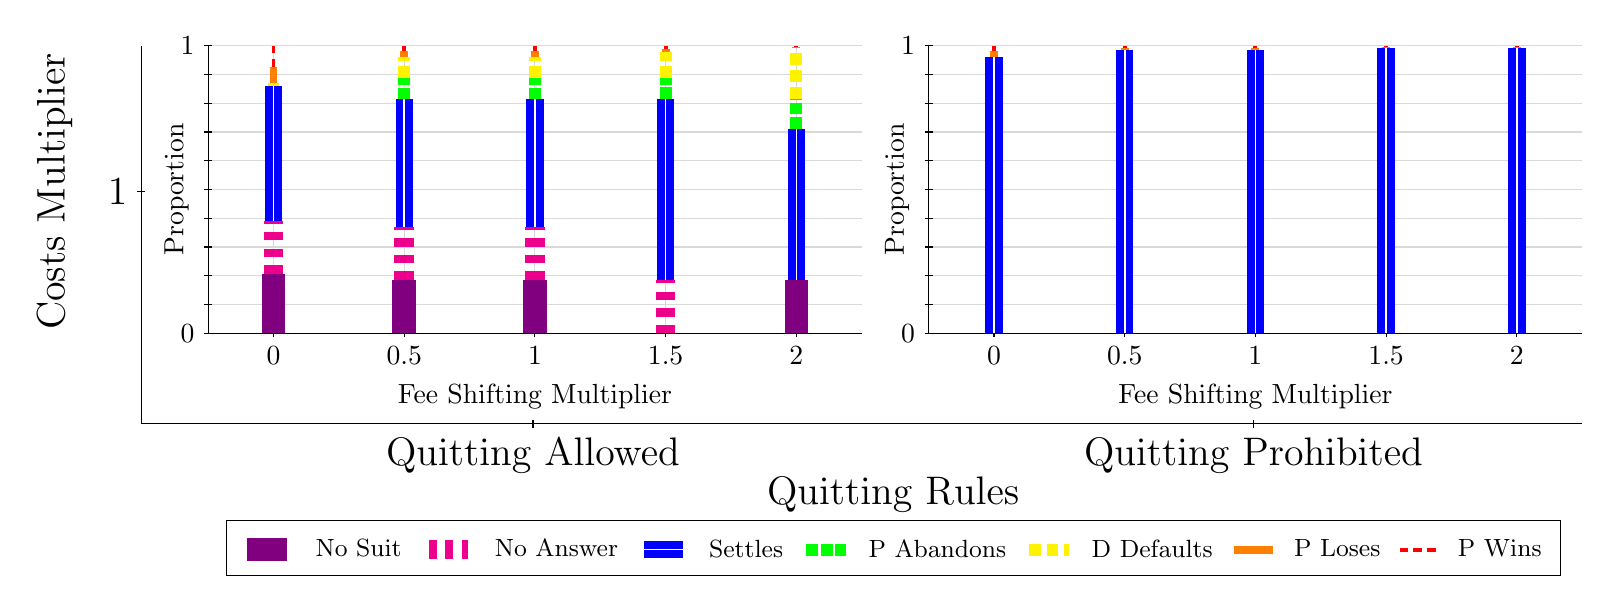
\begin{tikzpicture}
\draw[black] (1.7,1.5) -- (1.7,6.3);
\node[rotate=90, fontscale=2, anchor=center] at (0.6, 4.45) {Costs Multiplier};
\draw[black] (1.65,4.45) -- (1.75,4.45);
\node[fontscale=2, anchor=east] at (1.65, 4.45) {1};

\draw[black] (1.7,1.5) -- (20,1.5);
\node[fontscale=2, anchor=center] at (11.25, 0.6) {Quitting Rules};
\draw[black] (6.675,1.45) -- (6.675,1.55);
\node[fontscale=2, anchor=north] at (6.675, 1.45) {Quitting Allowed};
\draw[black] (15.825,1.45) -- (15.825,1.55);
\node[fontscale=2, anchor=north] at (15.825, 1.45) {Quitting Prohibited};


\draw[gray!30] (2.55,2.65) -- (10.85,2.65);
\draw[gray!30] (2.55,3.015) -- (10.85,3.015);
\draw[gray!30] (2.55,3.38) -- (10.85,3.38);
\draw[gray!30] (2.55,3.745) -- (10.85,3.745);
\draw[gray!30] (2.55,4.11) -- (10.85,4.11);
\draw[gray!30] (2.55,4.475) -- (10.85,4.475);
\draw[gray!30] (2.55,4.84) -- (10.85,4.84);
\draw[gray!30] (2.55,5.205) -- (10.85,5.205);
\draw[gray!30] (2.55,5.57) -- (10.85,5.57);
\draw[gray!30] (2.55,5.935) -- (10.85,5.935);
\draw[gray!30] (2.55,6.3) -- (10.85,6.3);
\draw[gray!30] (3.38,2.65) -- (3.38,6.3);
\draw[gray!30] (5.04,2.65) -- (5.04,6.3);
\draw[gray!30] (6.7,2.65) -- (6.7,6.3);
\draw[gray!30] (8.36,2.65) -- (8.36,6.3);
\draw[gray!30] (10.02,2.65) -- (10.02,6.3);
\draw[black] (2.55,2.65) -- (2.55,6.3);
\node[rotate=90, fontscale=0.7, anchor=center] at (2.15, 4.475) {Proportion};
\draw[black] (2.5,2.65) -- (2.6,2.65);
\node[fontscale=0.7, anchor=east] at (2.5, 2.65) {0};
\draw[black] (2.5,3.015) -- (2.6,3.015);
\node[fontscale=0.7, anchor=east] at (2.5, 3.015) { };
\draw[black] (2.5,3.38) -- (2.6,3.38);
\node[fontscale=0.7, anchor=east] at (2.5, 3.38) { };
\draw[black] (2.5,3.745) -- (2.6,3.745);
\node[fontscale=0.7, anchor=east] at (2.5, 3.745) { };
\draw[black] (2.5,4.11) -- (2.6,4.11);
\node[fontscale=0.7, anchor=east] at (2.5, 4.11) { };
\draw[black] (2.5,4.475) -- (2.6,4.475);
\node[fontscale=0.7, anchor=east] at (2.5, 4.475) { };
\draw[black] (2.5,4.84) -- (2.6,4.84);
\node[fontscale=0.7, anchor=east] at (2.5, 4.84) { };
\draw[black] (2.5,5.205) -- (2.6,5.205);
\node[fontscale=0.7, anchor=east] at (2.5, 5.205) { };
\draw[black] (2.5,5.57) -- (2.6,5.57);
\node[fontscale=0.7, anchor=east] at (2.5, 5.57) { };
\draw[black] (2.5,5.935) -- (2.6,5.935);
\node[fontscale=0.7, anchor=east] at (2.5, 5.935) { };
\draw[black] (2.5,6.3) -- (2.6,6.3);
\node[fontscale=0.7, anchor=east] at (2.5, 6.3) {1};

\draw[black] (2.55,2.65) -- (10.85,2.65);
\node[fontscale=0.7, anchor=center] at (6.7, 1.85) {Fee Shifting Multiplier};
\draw[black] (3.38,2.6) -- (3.38,2.7);
\node[fontscale=0.7, anchor=north] at (3.38, 2.6) {0};
\draw[black] (5.04,2.6) -- (5.04,2.7);
\node[fontscale=0.7, anchor=north] at (5.04, 2.6) {0.5};
\draw[black] (6.7,2.6) -- (6.7,2.7);
\node[fontscale=0.7, anchor=north] at (6.7, 2.6) {1};
\draw[black] (8.36,2.6) -- (8.36,2.7);
\node[fontscale=0.7, anchor=north] at (8.36, 2.6) {1.5};
\draw[black] (10.02,2.6) -- (10.02,2.7);
\node[fontscale=0.7, anchor=north] at (10.02, 2.6) {2};

\draw[violet, line width=3mm, solid] (3.38,2.65) -- (3.38,3.406);
\draw[violet, line width=3mm, solid] (5.04,2.65) -- (5.04,3.3292);
\draw[violet, line width=3mm, solid] (6.7,2.65) -- (6.7,3.3292);
\draw[violet, line width=3mm, solid] (8.36,2.65) -- (8.36,2.65);
\draw[violet, line width=3mm, solid] (10.02,2.65) -- (10.02,3.3292);
\draw[magenta, line width=2.5mm, dashed] (3.38,3.406) -- (3.38,4.0775);
\draw[magenta, line width=2.5mm, dashed] (5.04,3.3292) -- (5.04,4.0034);
\draw[magenta, line width=2.5mm, dashed] (6.7,3.3292) -- (6.7,4.0034);
\draw[magenta, line width=2.5mm, dashed] (8.36,2.65) -- (8.36,3.3291);
\draw[magenta, line width=2.5mm, dashed] (10.02,3.3292) -- (10.02,3.3292);
\draw[blue, line width=1mm, double] (3.38,4.0775) -- (3.38,5.7857);
\draw[blue, line width=1mm, double] (5.04,4.0034) -- (5.04,5.6195);
\draw[blue, line width=1mm, double] (6.7,4.0034) -- (6.7,5.6195);
\draw[blue, line width=1mm, double] (8.36,3.3291) -- (8.36,5.6207);
\draw[blue, line width=1mm, double] (10.02,3.3292) -- (10.02,5.2438);
\draw[green, line width=1.5mm, densely dotted] (3.38,5.7857) -- (3.38,5.7857);
\draw[green, line width=1.5mm, densely dotted] (5.04,5.6195) -- (5.04,5.8913);
\draw[green, line width=1.5mm, densely dotted] (6.7,5.6195) -- (6.7,5.8913);
\draw[green, line width=1.5mm, densely dotted] (8.36,5.6207) -- (8.36,5.8913);
\draw[green, line width=1.5mm, densely dotted] (10.02,5.2438) -- (10.02,5.6209);
\draw[yellow, line width=1.5mm, dotted] (3.38,5.7857) -- (3.38,5.8257);
\draw[yellow, line width=1.5mm, dotted] (5.04,5.8913) -- (5.04,6.163);
\draw[yellow, line width=1.5mm, dotted] (6.7,5.8913) -- (6.7,6.163);
\draw[yellow, line width=1.5mm, dotted] (8.36,5.8913) -- (8.36,6.2201);
\draw[yellow, line width=1.5mm, dotted] (10.02,5.6209) -- (10.02,6.2684);
\draw[orange, line width=1mm, solid] (3.38,5.8257) -- (3.38,6.0297);
\draw[orange, line width=1mm, solid] (5.04,6.163) -- (5.04,6.2315);
\draw[orange, line width=1mm, solid] (6.7,6.163) -- (6.7,6.2315);
\draw[orange, line width=1mm, solid] (8.36,6.2201) -- (8.36,6.2628);
\draw[orange, line width=1mm, solid] (10.02,6.2684) -- (10.02,6.2791);
\draw[red, line width=0.5mm, densely dashed] (3.38,6.0297) -- (3.38,6.3);
\draw[red, line width=0.5mm, densely dashed] (5.04,6.2315) -- (5.04,6.3);
\draw[red, line width=0.5mm, densely dashed] (6.7,6.2315) -- (6.7,6.3);
\draw[red, line width=0.5mm, densely dashed] (8.36,6.2628) -- (8.36,6.3);
\draw[red, line width=0.5mm, densely dashed] (10.02,6.2791) -- (10.02,6.3);

\draw[gray!30] (11.7,2.65) -- (20,2.65);
\draw[gray!30] (11.7,3.015) -- (20,3.015);
\draw[gray!30] (11.7,3.38) -- (20,3.38);
\draw[gray!30] (11.7,3.745) -- (20,3.745);
\draw[gray!30] (11.7,4.11) -- (20,4.11);
\draw[gray!30] (11.7,4.475) -- (20,4.475);
\draw[gray!30] (11.7,4.84) -- (20,4.84);
\draw[gray!30] (11.7,5.205) -- (20,5.205);
\draw[gray!30] (11.7,5.57) -- (20,5.57);
\draw[gray!30] (11.7,5.935) -- (20,5.935);
\draw[gray!30] (11.7,6.3) -- (20,6.3);
\draw[gray!30] (12.53,2.65) -- (12.53,6.3);
\draw[gray!30] (14.19,2.65) -- (14.19,6.3);
\draw[gray!30] (15.85,2.65) -- (15.85,6.3);
\draw[gray!30] (17.51,2.65) -- (17.51,6.3);
\draw[gray!30] (19.17,2.65) -- (19.17,6.3);
\draw[black] (11.7,2.65) -- (11.7,6.3);
\node[rotate=90, fontscale=0.7, anchor=center] at (11.3, 4.475) {Proportion};
\draw[black] (11.65,2.65) -- (11.75,2.65);
\node[fontscale=0.7, anchor=east] at (11.65, 2.65) {0};
\draw[black] (11.65,3.015) -- (11.75,3.015);
\node[fontscale=0.7, anchor=east] at (11.65, 3.015) { };
\draw[black] (11.65,3.38) -- (11.75,3.38);
\node[fontscale=0.7, anchor=east] at (11.65, 3.38) { };
\draw[black] (11.65,3.745) -- (11.75,3.745);
\node[fontscale=0.7, anchor=east] at (11.65, 3.745) { };
\draw[black] (11.65,4.11) -- (11.75,4.11);
\node[fontscale=0.7, anchor=east] at (11.65, 4.11) { };
\draw[black] (11.65,4.475) -- (11.75,4.475);
\node[fontscale=0.7, anchor=east] at (11.65, 4.475) { };
\draw[black] (11.65,4.84) -- (11.75,4.84);
\node[fontscale=0.7, anchor=east] at (11.65, 4.84) { };
\draw[black] (11.65,5.205) -- (11.75,5.205);
\node[fontscale=0.7, anchor=east] at (11.65, 5.205) { };
\draw[black] (11.65,5.57) -- (11.75,5.57);
\node[fontscale=0.7, anchor=east] at (11.65, 5.57) { };
\draw[black] (11.65,5.935) -- (11.75,5.935);
\node[fontscale=0.7, anchor=east] at (11.65, 5.935) { };
\draw[black] (11.65,6.3) -- (11.75,6.3);
\node[fontscale=0.7, anchor=east] at (11.65, 6.3) {1};

\draw[black] (11.7,2.65) -- (20,2.65);
\node[fontscale=0.7, anchor=center] at (15.85, 1.85) {Fee Shifting Multiplier};
\draw[black] (12.53,2.6) -- (12.53,2.7);
\node[fontscale=0.7, anchor=north] at (12.53, 2.6) {0};
\draw[black] (14.19,2.6) -- (14.19,2.7);
\node[fontscale=0.7, anchor=north] at (14.19, 2.6) {0.5};
\draw[black] (15.85,2.6) -- (15.85,2.7);
\node[fontscale=0.7, anchor=north] at (15.85, 2.6) {1};
\draw[black] (17.51,2.6) -- (17.51,2.7);
\node[fontscale=0.7, anchor=north] at (17.51, 2.6) {1.5};
\draw[black] (19.17,2.6) -- (19.17,2.7);
\node[fontscale=0.7, anchor=north] at (19.17, 2.6) {2};

\draw[violet, line width=3mm, solid] (12.53,2.65) -- (12.53,2.65);
\draw[violet, line width=3mm, solid] (14.19,2.65) -- (14.19,2.65);
\draw[violet, line width=3mm, solid] (15.85,2.65) -- (15.85,2.65);
\draw[violet, line width=3mm, solid] (17.51,2.65) -- (17.51,2.65);
\draw[violet, line width=3mm, solid] (19.17,2.65) -- (19.17,2.65);
\draw[magenta, line width=2.5mm, dashed] (12.53,2.65) -- (12.53,2.65);
\draw[magenta, line width=2.5mm, dashed] (14.19,2.65) -- (14.19,2.65);
\draw[magenta, line width=2.5mm, dashed] (15.85,2.65) -- (15.85,2.65);
\draw[magenta, line width=2.5mm, dashed] (17.51,2.65) -- (17.51,2.65);
\draw[magenta, line width=2.5mm, dashed] (19.17,2.65) -- (19.17,2.65);
\draw[blue, line width=1mm, double] (12.53,2.65) -- (12.53,6.163);
\draw[blue, line width=1mm, double] (14.19,2.65) -- (14.19,6.2416);
\draw[blue, line width=1mm, double] (15.85,2.65) -- (15.85,6.2416);
\draw[blue, line width=1mm, double] (17.51,2.65) -- (17.51,6.2684);
\draw[blue, line width=1mm, double] (19.17,2.65) -- (19.17,6.2684);
\draw[green, line width=1.5mm, densely dotted] (12.53,6.163) -- (12.53,6.163);
\draw[green, line width=1.5mm, densely dotted] (14.19,6.2416) -- (14.19,6.2416);
\draw[green, line width=1.5mm, densely dotted] (15.85,6.2416) -- (15.85,6.2416);
\draw[green, line width=1.5mm, densely dotted] (17.51,6.2684) -- (17.51,6.2684);
\draw[green, line width=1.5mm, densely dotted] (19.17,6.2684) -- (19.17,6.2684);
\draw[yellow, line width=1.5mm, dotted] (12.53,6.163) -- (12.53,6.163);
\draw[yellow, line width=1.5mm, dotted] (14.19,6.2416) -- (14.19,6.2416);
\draw[yellow, line width=1.5mm, dotted] (15.85,6.2416) -- (15.85,6.2416);
\draw[yellow, line width=1.5mm, dotted] (17.51,6.2684) -- (17.51,6.2684);
\draw[yellow, line width=1.5mm, dotted] (19.17,6.2684) -- (19.17,6.2684);
\draw[orange, line width=1mm, solid] (12.53,6.163) -- (12.53,6.2315);
\draw[orange, line width=1mm, solid] (14.19,6.2416) -- (14.19,6.2708);
\draw[orange, line width=1mm, solid] (15.85,6.2416) -- (15.85,6.2708);
\draw[orange, line width=1mm, solid] (17.51,6.2684) -- (17.51,6.2791);
\draw[orange, line width=1mm, solid] (19.17,6.2684) -- (19.17,6.2791);
\draw[red, line width=0.5mm, densely dashed] (12.53,6.2315) -- (12.53,6.3);
\draw[red, line width=0.5mm, densely dashed] (14.19,6.2708) -- (14.19,6.3);
\draw[red, line width=0.5mm, densely dashed] (15.85,6.2708) -- (15.85,6.3);
\draw[red, line width=0.5mm, densely dashed] (17.51,6.2791) -- (17.51,6.3);
\draw[red, line width=0.5mm, densely dashed] (19.17,6.2791) -- (19.17,6.3);

\draw (11.25,0) node[draw=none] (baseCoordinate) {};
\begin{scope}[align=center]
        \matrix[scale=0.5, draw=black, below=-0.4cm of baseCoordinate, nodes={draw}, column sep=0.1cm]{
        
\draw[violet, line width=3mm, solid] (0.25,-0.25) -- (0.75,-0.25); &
\node[draw=none, font=\small] (B) {No Suit}; &

\draw[magenta, line width=2.5mm, dashed] (0.25,-0.25) -- (0.75,-0.25); &
\node[draw=none, font=\small] (B) {No Answer}; &

\draw[blue, line width=1mm, double] (0.25,-0.25) -- (0.75,-0.25); &
\node[draw=none, font=\small] (B) {Settles}; &

\draw[green, line width=1.5mm, densely dotted] (0.25,-0.25) -- (0.75,-0.25); &
\node[draw=none, font=\small] (B) {P Abandons}; &

\draw[yellow, line width=1.5mm, dotted] (0.25,-0.25) -- (0.75,-0.25); &
\node[draw=none, font=\small] (B) {D Defaults}; &

\draw[orange, line width=1mm, solid] (0.25,-0.25) -- (0.75,-0.25); &
\node[draw=none, font=\small] (B) {P Loses}; &

\draw[red, line width=0.5mm, densely dashed] (0.25,-0.25) -- (0.75,-0.25); &
\node[draw=none, font=\small] (B) {P Wins}; \\
            };
\end{scope}

\end{tikzpicture}
\end{document}